% TODO:
% - Make a tool for download and transformation of datasets, and sell the work that I have done
% - Compare single user datasets
% - group rec datasets mention
% - do dataset group augmentation and add it to the tool


\chapter{Datasets}  \label{chap:datasets}
People are gregarious in nature, but the same, unfortunately, cannot be said about machine learning datasets. The vast majority of them are not directly usable in the group RS research due to only containing information about single-user preferences. To design and evaluate group recommender systems, we preferably need datasets that contain information about groups' preferences.

In this chapter, we will describe which datasets are suitable for use in the RS domain. We describe commonly used datasets in the non-group RS domain. Then, we analyze their high-level properties and describe what transformations are needed to make the dataset convenient to use. 

Next, we will talk about the existing group RS datasets and introduce methods that can be used to generate the group recommendation information synthetically from non-group RS datasets. We will use these methods to generate standardized synthetically enriched group RS datasets from non-group datasets that we describe in the single-user datasets subchapter.

% And finally, we describe a data transformation library that we created for the purpose of simplifying the research efforts in the RS domain and for the evaluation of our proposed algorithm.

% We will first describe a few of the popular datasets which we have determined to be used as research data the most. Then we will 

% -------------------------------------------------------------------------------------
\section{Single user datasets} \label{sec:single_user_datasets}
% -------------------------------------------------------------------------------------
Multiple well-known and thoroughly studied datasets exist in the recommender system domain. Let us present the popular ones that seem to be utilized the most.

When we talk about the specific format of the data, then we are referring to the unified format which we have transformed the original data into using the dataset transformation library. Further description of the data format transformations follows in Subsection \ref{subsec:04_single_user_datasets.gathering_processing}.



% -------------------------------------------------------------------------------------
\subsection{Movie Lens}
% -------------------------------------------------------------------------------------
One of the most well-known datasets in the RS domain, it contains 25 million ratings in total across 62,000 movies and 162,000 users. The data were collected between 1995 and 2019, and the current version of this size (25M) was released in November of 2019. Data are organic and come from a web-based recommendation system at \href{https://movielens.org/}{movielens.org}. The project was specifically created in order to gather research data on personalized recommendations by researchers at the University of Minnesota.

The dataset is in a suitable format that is easy to parse and use. A further description follows in Subsection \ref{subsec:04_single_user_datasets.gathering_processing}.

\hfill \break
\noindent
\textbf{Number of items:} 62,000 \newline
\textbf{Number of users:} 162,000 \newline
\textbf{Number of user-item interactions:} 25,000,095 \newline
\textbf{User-item interactions format:} Sparse matrix of ordinal ratings [1, 1.5, 2, ... 4.5, 5] - user rated a movie \newline
\textbf{List of data tables:} Movies (detail in Table \ref{table:5.1_ML_movies}), Ratings (detail in Table \ref{table:5.1_ML_ratings}), Tags, Links, Genres, Genome Scores, Genome Tags

\begin{table}[ht!]
\centering
\begin{tabular}{ l l }
\verb|item_id| & \verb|title| \\
    \hline
     1  &                   Toy Story (1995) \\
     2  &                     Jumanji (1995) \\
     3  &            Grumpier Old Men (1995) \\
   ...  &                                ... \\
209169  &                A Girl Thing (2001) \\
209171  &     Women of Devil's Island (1962) \\ [1mm]
\multicolumn{2}{l}{{[62423 rows x 2 columns]}}
\end{tabular}
\caption{Short snippet of Movie Lens dataset's \texttt{movies.csv} table.}
\label{table:5.1_ML_movies}
\end{table}

\begin{table}[!ht]
\centering
\begin{tabular}{ l l l l }


\verb|user_id| & \verb|item_id| & \verb|rating| & \verb|timestamp| \\
    \hline
    1 &      296  &   5.0 & 1147880044 \\
    1 &      306  &   3.5 & 1147868817 \\
    1 &      307  &   5.0 & 1147868828 \\
  ... &      ...  &   ... &        ... \\
162541 &    58559  &   4.0 & 1240953434 \\
162541 &    63876  &   5.0 & 1240952515 \\ [1mm]
\multicolumn{4}{l}{{[25000095 rows x 4 columns]}}
\end{tabular}
\caption{Short snippet of Movie Lens dataset's \texttt{ratings.csv} table.}
\label{table:5.1_ML_ratings}
\end{table}




% -------------------------------------------------------------------------------------
\subsection{KGRec}
\label{subsec:04_single_user_datasets.kgrec}
% -------------------------------------------------------------------------------------
KGRec is a smaller and less known dataset. We have chosen this dataset because it was utilized in the GFAR method introduced in \cite{GFAR-kaya2020} and described in Subsection \ref{subsec:03_advanced_methods.gfar}. This dataset consists of two separate datasets of music and sound, KGRec-music and KGRec-sound, respectively.

The first music dataset comes from \href{https://www.songfacts.com/}{songfacts.com} (items and text descriptions) and \href{https://www.last.fm/}{last.fm} (ratings, items, tags). Each user-item interaction is a user listening to a song.

The second sound dataset comes from \href{https://freesound.org/}{freesound.org}. Items are sounds with descriptions using text and tags created by the person who uploaded the sound. Each user-item interaction is a user downloading an item, in this case, a sound.

Further, we will consider only the music dataset and not utilize the sound dataset. We have made this decision to simplify comparisons due to the origin of the sound dataset itself. It comes from a web page where users can upload and download random sounds of their choosing, such as the 'Mechanical clock movement' sound, 'Industrial elevator' sound, and other. The need for these sounds is most probably driven by people using them for their profession, such as video production, and therefore does not reflect natural content consumption preferences.

Both datasets were created for the needs of \cite{kgrec_dataset_origin}, where they were introduced, and they are altered for the needs of research in Recommendation Knowledge Graphs. Further, the original data that was used for the creation of these datasets are described in \cite{kgrec_dataset_origin_full}.


\hfill \break
\noindent
\textbf{Number of items:} 8,640; 21,552\footnote{All KGRec statistics are in order - music dataset; sound dataset} \newline
\textbf{Number of users:} 5,199; 20,000 \newline
\textbf{Number of user-item interactions:} 751,531; 2,117,698 \newline
\textbf{User-item interactions format:} one-valued implicit feedback - user listened or downloaded a song/sound \newline
\textbf{List of data tables:} Ratings(detail in Table \ref{table:5.1_KGRec_ratings}), Tags, Descriptions

\begin{table}[!ht]
    \centering
    \begin{tabular}{ l l }
        \verb|user_id|   & \verb|item_id| \\
        \hline
        7596     &  68  \\
        7596     & 130  \\
        7596     & 330  \\
        ...      & ...  \\
        50572897 & 8618 \\
        50572897 & 8619 \\ [1mm]
        \multicolumn{2}{l}{{[751531 rows x 2 columns]}}
    \end{tabular}
    \caption{Short snippet of KGRec dataset's \texttt{music\_ratings.csv} table.}
    \label{table:5.1_KGRec_ratings}
\end{table}

% \newline
% Both dataset are in the form of '\textlessuser userId, itemId\textgreater'


% -------------------------------------------------------------------------------------
\subsection{Netflix Prize}
% -------------------------------------------------------------------------------------

Data that were originally released in 2009 by the Netflix.com video streaming company for the \textit{Netflix Prize}, an open competition with the main prize of 1 million dollars. It contains data from more than 400 thousand randomly selected users from the company's database. Data contain information about users' ratings of movies. It was originally available on the contest web page but has been removed.

The original data was split into multiple files in a file for ratings per movie manner. Each rating is a quadruplet of the form '\textless user, movie, date of the rating, rating\textgreater'.

\hfill \break
\noindent
\textbf{Number of items:} 17,770 \newline
\textbf{Number of users:} 480,189 \newline
\textbf{Number of user-item interactions:} 100,480,507 \newline
\textbf{User-item interactions format:} sparse matrix of ordinal ratings [1, 2, 3, 4, 5] \newline
\textbf{List of data tables:} Ratings (detail in Table \ref{table:5.1_Netflix_ratings}), Movies (detail in Table \ref{table:5.1_Netflix_movies})

\begin{table}[!ht]
    \centering
    \begin{tabular}{ l l l l }
        \verb|user_id| & \verb|item_id| & \verb|rating| & \verb|date| \\
        \hline
              6 &             30 &             3 &  2004-09-15 \\
              6 &            157 &             3 &  2004-09-15 \\
              6 &            173 &             4 &  2004-09-15 \\
            ... &            ... &           ... &         ... \\
        2649429 &          17627 &             3 &  2003-07-21 \\
        2649429 &          17692 &             2 &  2002-12-07 \\ [1mm]
        \multicolumn{4}{l}{{[100480507 rows x 4 columns]}}
    \end{tabular}
    \caption{Short snippet of Netflix dataset's \texttt{ratings.csv} table.}
    \label{table:5.1_Netflix_ratings}
\end{table}
    
\begin{table}[!ht]
    \centering
    \begin{tabular}{ l l l }
        \verb|item_id| & \verb|release_year| & \verb|title| \\
        \hline
            1 &       2003.0 &            Dinosaur Planet    \\
            2 &       2004.0 & Isle of Man TT 2004 Review    \\
            3 &       1997.0 &                  Character    \\
          ... &          ... &                        ...    \\
        17769 &       2003.0 &                The Company    \\
        17770 &       2003.0 &               Alien Hunter \\ [1mm]
        \multicolumn{3}{l}{{[17770 rows x 3 columns]}}
    \end{tabular}
    \caption{Short snippet of Netflix dataset's \texttt{movies.csv} table.}
    \label{table:5.1_Netflix_movies}
\end{table}
% -------------------------------------------------------------------------------------
\subsection{Spotify - Million Playlist Dataset}
% -------------------------------------------------------------------------------------
This dataset was released in January 2018 for \textit{The Spotify Milion Playlist Dataset Challenge}. It contains 1,000,000 playlists with information about tracks that are part of each playlist. The primary purpose of this dataset was to study and develop better algorithms for automatic playlist continuation where the system could recommend songs that are similar to those already in the playlist. In contrast to the Netflix challenge, no prize was to be awarded at the end of the challenge.

Even though the context of this dataset is playlists and not users, we utilize a different view of the dataset, where each playlist will represent a single user. This way, we have another big and organic dataset at our disposal. It can therefore be used not only for playlist continuation tasks but also for the classical RS domain tasks. In a sense, a single playlist is a specific subset of the user's preference that has created the playlist. Therefore we expect to see a narrower preference distribution for each of these 'playlist' users.

For completeness, it is necessary to add that some playlists are 'collaborative', meaning that they were created by multiple users. Nevertheless, they account for only 2.3\% of all playlists, which in our opinion, does not substantially affect the dataset. These collaborative datasets could be used as a group recommender dataset on their own. Unfortunately, the information about which user added which track to the collaborative playlist is not present.

\begin{table}[!ht]
    \centering
    \begin{tabular}{ l l }
        \verb|playlist_id|   & \verb|item_id| \\
        \hline
        549000     &  0  \\
        549000     & 1  \\
        549000     & 2  \\
        ...      & ...  \\
        302999 & 133087 \\
        302999 & 133088 \\ [1mm]
        \multicolumn{2}{l}{{[66346428 rows x 2 columns]}}
    \end{tabular}
    \caption{Short snippet of Spotify Milion Playlist dataset's \texttt{ratings.csv} table.}
    \label{table:5.1_Spotify_ratings}
\end{table}


\begin{table}[!ht]
    \centering
    \begin{tabular}{ l l l }
        \verb|item_id| & \verb|item_name| & \verb|artist_name|  \\
        \hline
             0 & Boots of Spanish Leather &         Bob Dylan \\
             1 &       Mr. Tambourine Man &         Bob Dylan \\
             2 &             Danny's Song & Loggins \& Messina \\ 
           ... &                      ... &               ... \\
       2262290 &               Robin Hood &        Crazy Fool \\
       2262291 &                Guilttrip &      Ace Reporter \\ [1mm]
       \multicolumn{3}{l}{{[2262292 rows x 6 columns]}}
    \end{tabular}
    \caption[Short snippet of Netflix dataset's \texttt{tracks.csv} table.]{Short snippet of Netflix dataset's \texttt{tracks.csv} table. (Columns \texttt{item\_uri}, \texttt{artist\_uri}, \texttt{album\_uri}, containing URI to Spotify object were omitted for simplicity due to their substantial length.)}
    \label{table:5.1_Spotify_tracks}
\end{table}

\hfill \break
\noindent
\textbf{Number of items:} 2,262,292 \newline
\textbf{Number of users:} 1,000,000 \newline
\textbf{Number of user-item interactions:} 66,346,428 \newline
\textbf{User-item interactions format:} one-valued implicit feedback - user added a song to a playlist\newline
\textbf{List of data tables:} Tracks (detail in Table \ref{table:5.1_Spotify_tracks}), Ratings (detail in Table \ref{table:5.1_Spotify_ratings})




% -------------------------------------------------------------------------------------
\subsection{Comparison of datasets}
% -------------------------------------------------------------------------------------

\begin{figure}[ht!]
    \centering
    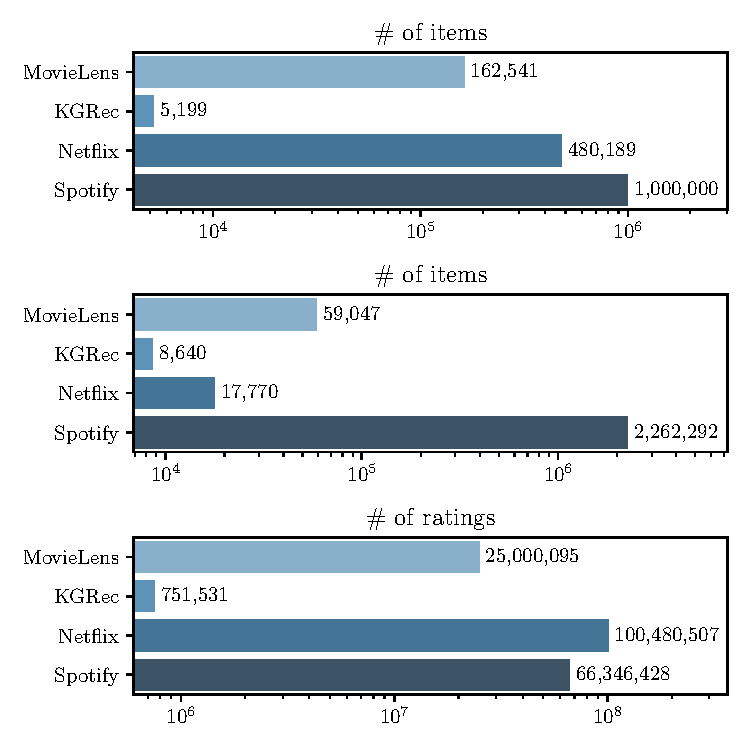
\includegraphics{img/figures/datasets_counts.pdf}
    \caption[Size comparison of the selected datasets.]{Size comparison of the selected datasets. All x-axes are log scales due to the big differences between the dataset.}
    \label{fig:datasets_counts}
\end{figure}

We have described each dataset separately. Let us now compare them together to see how they differ. As shown in Figure \ref{fig:datasets_counts}, the Spotify and Netflix datasets are the biggest. We see that the KGRec dataset is almost two orders of magnitude smaller than the rest. As already mentioned, we have selected it due to its common utilization in the related literature. Spotify dataset is different by having two orders of magnitude more items, which can present a challenge on its own. For example, if we use matrix factorization methods to compute the preference, then the amount of memory will rise by two orders of magnitude as well. Additionally, the sparsity of ratings is higher, which can negatively affect efficacy.

The Movie Lens dataset has a potential benefit as it has actual ratings for each user-item interaction. All other presented datasets only contain user-item interactions in the form of one-valued implicit feedback.

\begin{figure}[htbp!]
    \centering
    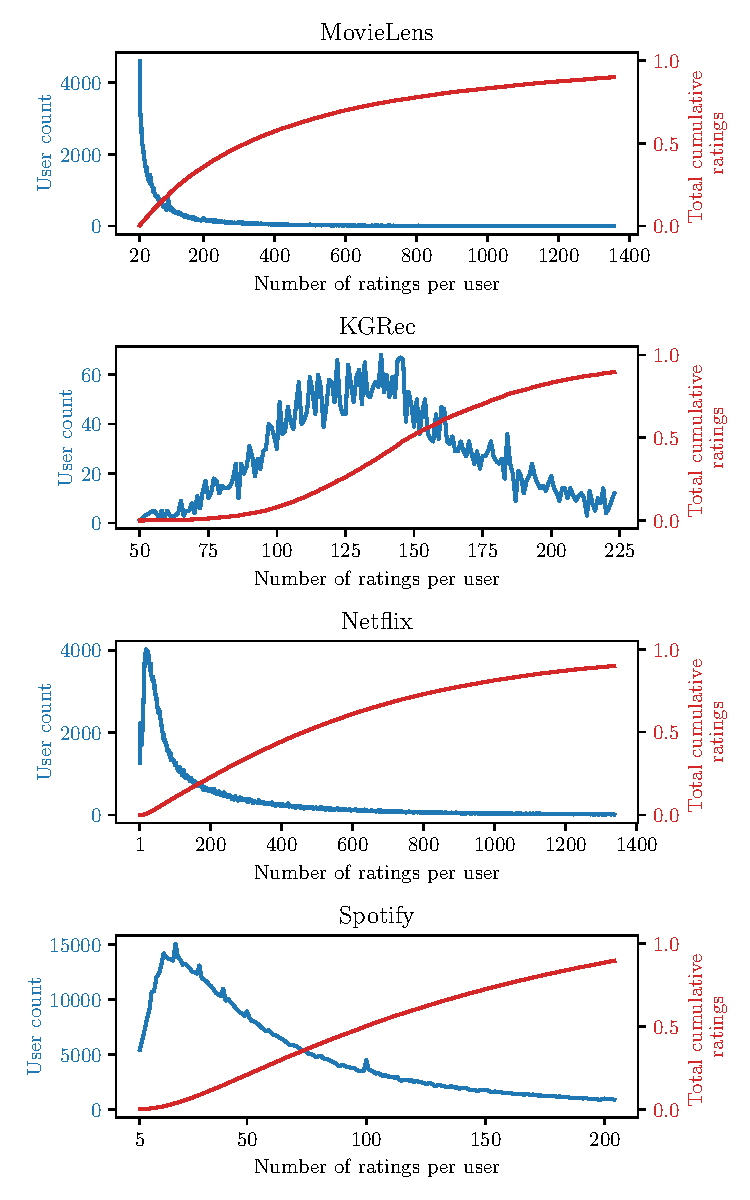
\includegraphics{img/figures/num_users_by_rating_count.pdf}
    \caption[Distribution of ratings]{Distribution of ratings for groups of users by how many ratings they have made. The blue line shows how many users have made that particular amount of ratings, while the red line shows the total cumulative mass distribution of ratings. We have clipped the number of ratings by total cumulative ratings of 90\% due to very long-tailed data, where some small amount of users created a very high amount of ratings.}
    \label{fig:datasets_num_ratings}
\end{figure}

In Figure \ref{fig:datasets_num_ratings}, we present the distribution of ratings among users. The left y-axis, blue, presents the count of users with a particular number of ratings. We have clipped the users with a high number of ratings so that we can better see the interesting part of the data, which the long tails would otherwise squash. The clip was made on the last 10\% mass of all ratings.

We see that Movie Lens nicely follows a power-law distribution. In this dataset, only users with more than 20 ratings are present, which is also visible in the figure and is most probably why we do not see the same initial rise in ratings as for Netflix and Spotify datasets'.

The KGRec dataset is different. It is more jagged due to the smaller effect of being smoothed out by the amount of data as with the other datasets. Interestingly, the number of users does not follow an exponential distribution in contrast to the other datasets. At first, we thought the reason was that the dataset was gathered at a website where users listen and download songs. These songs are always a part of an album; if a user is downloading one song from an album, they will most likely also download the rest of the album. However, that would not explain why this number of ratings per user starts at around 75.

The actual reason for this can be partially found in the original paper - \cite{kgrec_dataset_origin}. As already described in Subsection \ref{subsec:04_single_user_datasets.kgrec}, the dataset was altered to better fit the required research objective of recommendation using knowledge graphs. As such, songs with less than ten interactions have been removed, users with less than 50 item interactions have been removed, and only songs with over-average plays were counted as user-item interactions. Nevertheless, this would not explain the nonexponential nature of the distribution. We have downloaded and explored the original dataset from \cite{kgrec_dataset_origin_full}, the original dataset is not only one-valued implicit feedback, but it is the number of times a user has played the song. When we visualize the original dataset using the 'sum of plays per user' instead of the 'count of interactions per user', we get a natural-looking exponential distribution. Therefore, the most probable reason for the KGRec's dataset distribution is that users like to replay a smaller number of songs multiple times, creating more of a normal-looking distribution.

Further, the Netflix dataset looks similar to Movie Lens, with two exceptions. The first is that Movie Lens includes only users with at least 20 ratings. Therefore the initial increase in the number of ratings is not visible. Secondly, both Netflix and Spotify datasets have cumulative rating distribution shifted more to the right, which means that there are more ratings among users that were more active on the service and interacted with many items.




% -------------------------------------------------------------------------------------
\subsection{Datasets gathering and processing} \label{subsec:04_single_user_datasets.gathering_processing}
% -------------------------------------------------------------------------------------

Processing the datasets mentioned above was more difficult than it should have been. They are not easily accessible. Some are available only behind a login wall and in different, incompatible, and non-standard formats. We have therefore processed and unified these datasets using a tool that we have developed. At first, we wanted to create shared storage where they would be available in the already transformed form, but that is not feasible due to the datasets' licenses. Let us now describe the data transformations we have done for each dataset. We aim to have the datasets in standard zipped CSV format that can be simply loaded by most of the widespread data manipulation tools such as Pandas. Additionally, if not misleading, we prefer the columns of the datasets to be named in a unified fashion.

\begin{itemize}
    \item \textbf{Movie Lens} dataset is available at the the authors web page \newline \href{https://grouplens.org/datasets/movielens/25m/}{grouplens.org/datasets/movielens/25m/}. This dataset is easily accessible and ready-to-be-used (files in valid CSV format, zipped together in a single archive). This was the nicest dataset to start working with. No transformations were necessary apart from remapping user and item ids to be sequential.
    
    \item \textbf{KGRec} dataset is available for download at the authors web page\newline \href{https://www.upf.edu/web/mtg/kgrec}{upf.edu/web/mtg/kgrec}. Unfortunately, downloading the dataset is not straightforward because the download link is an unsecured HTTP on a secured HTTPS site. This is a problem while using modern browsers, which do not support mixed HTTP and HTTPS content. The dataset has ratings in a standard CSV form with redundant information about the incidence, which is always of value 1. Main data in sparse incidence matrix representation are in the form of '\textless userId, itemId\textgreater'. Additional data with tags and descriptions of items are separated into individual files in the original dataset. We have transformed them into two CSV tables of form '\textless itemId, tags\textgreater' and '\textless movieId, description\textgreater' respectively. Further, remapping of user and item ids to sequential values was performed.
    \item \textbf{Netflix} dataset is available on an independent web page
    \newline
    \href{https://www.kaggle.com/datasets/netflix-inc/netflix-prize-data}{kaggle.com/datasets/netflix-inc/netflix-prize-data}.
    The original web page of the challenge is no longer available. The uploader additionally processed the dataset by aggregating the small per-movie rating files into four bigger files. This dataset was in a non-standard format where ratings were not in CSV but in a custom format reflecting the original movie ratings per file division. Each group of ratings for a movie starts with a line only containing the id of the movie and a colon, then ratings for the movie follow each per line in a format '\textless user-id,rating,timestamp\textgreater'.
    
    \item \textbf{Spotify} dataset is available at AIcrowd.com, where the original Spotify challenge was introduced. Unfortunately, the dataset is behind a login wall. After registering and logging in, it can be downloaded from \newline\href{https://www.aicrowd.com/challenges/spotify-million-playlist-dataset-challenge}{aicrowd.com/challenges/spotify-million-playlist-dataset-challenge}.
    
    
    The dataset is comprised of 1000 JSON files, each describing 1000 playlists. The dataset contains a lot of information about each playlist such as the name, when it was modified, how many followers it has, and so on. We go through all data and simultaneously create a list of playlists to track mapping and another list with any additional track information, such as the Spotify URI links for the track, album, and artist. We have created a separate numerical track id due to the native one of the track URI being too long. Apart from the JSON files, the zip archive contains some python code to provide easy parsing and simple statistics about the dataset.
    
\end{itemize}


% todo: pocet ratingu
% srovnat itemy podle toho kolik lidi hodnotilo a zobrazit prumerny rating



We have created a Python CLI tool that can be used to download the available datasets easily. This tool is available in our Git repository at \newline\href{https://github.com/LadislavMalecek/MasterThesisAnalysis}{github.com/LadislavMalecek/MasterThesisAnalysis}. Run \path{./gather_datasets/download_and_transform.py} to execute the script. All relevant information about the supported parameters is available when run with the standard '--help' switch.


% -------------------------------------------------------------------------------------
\section{Group datasets}
% -------------------------------------------------------------------------------------
Let us now investigate datasets that contain information about groups of users. We will look through some of the datasets mentioned in related literature.

\subsection{Datasets overview}\label{subsection:04_}

When reading through related literature on GRS, we have mostly encountered synthetically created datasets either from the Movie Lens dataset or the Netflix dataset. The main reason for not utilizing datasets with innate group information is that not many of them exist. Let us go through some of the datasets mentioned in the related literature and determine their suitability for group recommender system research.

First, we would like to point out a critical flaw that most literature in our domain has. Suppose the authors decide to use some small, unknown, and or proprietary dataset, instead of using the traditional Movie Lens and Netflix datasets. Then for the research reproducibility, it is necessary to provide a detailed description about where and how the dataset can be obtained and how the raw dataset was created, filtered, and altered. Most authors do not mention these details and only mention which dataset they were using and some high-level information about the dataset, such as the number of users, items, and interactions. This makes the papers' experiments irreproducible and unverifiable. The same can sometimes be said about papers that use single-user datasets with synthetically generated group information. Sometimes, it is not entirely clear how the synthetic groups have been generated and to what values the parameters have been set.

In Table \ref{table:5.2_GRS_datasets_comparation}, we present a high-level overview of datasets that we found in the related literature.

\begin{table}[!ht]
    \centering
    \begin{tabular}{ r | c c c c }
         & \#users & \#items & \#groups & avg. g. size \\
        \hline
            CAMRa2011\cite{attentative_group_recommendation}
                & 602 & 7,710 & 290 & ? \\
            Douban\cite{gowalla_weeplaces_yelp}
                & 23,032 & 10,039 & 58,983 & 4.2 \\
            Gowalla\cite{gowalla_weeplaces_yelp}
                & 25,405 &  38,306 & 44,565 &  2.8 \\
            Mafengwo\cite{attentative_group_recommendation}
                & 5,275 & 1,513 & 995 & ? \\
            Meetup\cite{meetup_origin}
                & 42,747 & 2,705 & 13,390 & 16.66 \\
            Plancast\cite{meetup_plancast}
                & 41,065 & 13,514 & 25,447 & 12.01 \\
            Yelp\cite{gowalla_weeplaces_yelp}
                & 7,037 & 7,671 & 10,214 & 6.8 \\
            Weeplaces\cite{gowalla_weeplaces_yelp}
                &  8,643 & 25,081 & 22,733 & 2.9 \\
    \end{tabular}
    \caption[Size overview of selected GRS datasets]{Size overview of selected GRS datasets. Note: Some dataset sizes are given after transforming the original datasets by removing users and items that are not part of any group.}
    \label{table:5.2_GRS_datasets_comparation}
\end{table}


\subsubsection{CAMRa2011} \label{subsubsec:04_group_datasets.overview.camra}
The CAMRa2011 dataset was released in 2011 for the 2011 ACM Recommender Systems Conference. The dataset is unavailable at the original location, and we could not retrieve it from the web. Numbers in Table \ref{table:5.2_GRS_datasets_comparation} are taken from \cite{attentative_group_recommendation}. We have found an altered version of the dataset at \newline \href{https://github.com/LianHaiMiao/Attentive-Group-Recommendation}{github.com/LianHaiMiao/Attentive-Group-Recommendation}, which is a GitHub repository for the code and experiments from \cite{attentative_group_recommendation}. The dataset is quite small and we are doubtful about its quality and source.


\subsubsection{Douban} \label{subsubsec:04_group_datasets.overview.douban}
This dataset has similar problems to the CAMRa2011 dataset. We were unable to retrieve it from the web. At the same time, in the already mentioned repository for \cite{attentative_group_recommendation}, we found an author's comment about adding the dataset soon (in 2018), which was never done.


\subsubsection{Gowalla} \label{subsubsec:04_group_datasets.overview.gowalla}
Gowalla was a location-based social network. It was dissolved in 2012 when Facebook acquired it. The dataset contains people logging in to locations that they have visited. The dataset can be easily downloaded at \href{https://www.yongliu.org/datasets/}{yongliu.org/datasets/}. We have discovered this page and dataset in \cite{gowalla_weeplaces_yelp}.

This dataset does not directly contain any group information. However, it could be inferred by combining the check-in data in the format '\textless userId, placeId, datetime\textgreater' and friendship data that link pairs of users '\textless userid1, userid2\textgreater'. If a person and some of their friends visit the same place around the same time, we can state that they were probably all part of the same group. Moreover, if they visit multiple places together, then the chance of a random occurrence drops significantly.

We suspect that there will be a substantial location similarity bias due to the data being location-based. If someone visits a specific place, they are very likely to visit a popular place nearby regardless of its quality.

\begin{itemize}
    \item \textbf{Available group information:} No explicit information, but group information can be interpolated from information about friendships and user-item interaction timestamps
    \item \textbf{User-item interactions:} one-valued implicit feedback
    \item \textbf{Group-item interactions:} none
    \item \textbf{Items type:} points-of-interests
\end{itemize}


\subsubsection{Mafengwo} \label{subsubsec:04_group_datasets.overview.mafengwo}
Tiny and proprietary dataset mentioned in \cite{attentative_group_recommendation}. The dataset is unavailable for download. We were unable to find another source from which we would be able to download this dataset.


\subsubsection{Meetup} \label{subsubsec:04_group_datasets.overview.meetup}
This dataset is crawled data from website \href{https://www.meetup.com}{meetup.com} from \cite{meetup_origin} used in \cite{meetup_plancast}. Meetup is a popular web page for meeting other people with similar hobbies and interests. This dataset contains only data from two regions, New York City and the state of California. One substantial distinction from other datasets is that the items represent non-repeating social events. This creates difficulties with similarity calculation between users due to the low average number of user-item interactions per item. Groups are defined explicitly with the grouping function, and members can communicate within the group and attend events or plan events together.

With some difficulties, we have downloaded the dataset from
\newline\href{https://personal.ntu.edu.sg/gaocong/datacode.htm}{personal.ntu.edu.sg/gaocong/datacode.htm}.

\begin{itemize}
    \item \textbf{Available group information:} group memberships, groups are on average big
    \item \textbf{User-item interactions:} one-valued implicit feedback
    \item \textbf{Group-item interactions:} none
    \item \textbf{Items type:} social events
\end{itemize}


\subsubsection{Plancast} \label{subsubsec:04_group_datasets.overview.plancast}
Unfortunately, we were unable to obtain this dataset for further analysis. In \cite{meetup_plancast}, where this dataset is mentioned, there is no download link, only a reference to \cite{plancast_origin}, where no additional information about the source is provided.

\subsubsection{Yelp}\label{subsubsec:04_group_datasets.overview.yelp}
This dataset contains reviews for businesses and places. In \cite{gowalla_weeplaces_yelp}, they use a subset of the whole dataset only for the city of Los Angeles. The whole dataset can be downloaded at \href{https://www.yelp.com/dataset}{yelp.com/dataset} and, in its unfiltered variant, is vastly bigger than other mentioned datasets with over 6,9 million ratings.

\begin{itemize}
    \item \textbf{Available group information:} no explicit information, but group information can be interpolated from friendships and user-item interaction's timestamps
    \item \textbf{User-item interactions:} one-valued implicit feedback and text reviews
    \item \textbf{Group-item interactions:} none
    \item \textbf{Items type:} Points-of-interests
\end{itemize}


\subsubsection{Weeplaces} \label{subsubsec:04_group_datasets.overview.weeplaces}
Similarly to the Gowalla dataset, Weeplaces was a website that aimed to visualize users' location-based check-in activities. It has been integrated with multiple location-based social networking services such as Foursquare and Facebook.
It contains information about check-ins and friendships, the same as the Gowalla dataset. It can be downloaded from \href{https://www.yongliu.org/datasets/}{yongliu.org/datasets/}. We have discovered this page and dataset in \cite{gowalla_weeplaces_yelp}.
Again, the same arguments for the group information and location-based bias hold for this dataset, the same as for the Gowalla dataset. 

How groups are created is not described in the original paper. Other information which is missing is a complete description of how was the raw dataset transformed and filtered. A high-level description is present, but it is incomplete.


\begin{itemize}
    \item \textbf{Available group information:} none explicit, can be interpolated from friendship information and user-item interaction timestamps
    \item \textbf{User-item interactions:} one-valued implicit feedback
    \item \textbf{Group-item interactions:} none
    \item \textbf{Items type:} Places check-ins
\end{itemize}


\subsubsection{Dataset selection}
Let us now select a subset of the mentioned datasets for further analysis and for inclusion in our download and transform tool.

We have rated all datasets on a scale of 'poor', 'ok', and 'good' in Table \ref{table:5.2_GRS_datasets_rating} for the following important criteria:
\begin{itemize}
    \item \textbf{Ease of retrieval} \newline
        We award a 'poor' rating if the dataset cannot be downloaded at all. Award an 'ok' rating if we can download the dataset with some difficulties from either the source in the mentioned paper or any related linked papers, as well as if we can download the dataset from an unrelated source. We award a 'good' rating if the dataset is easily downloadable using the original sources or any source original to the dataset, such as the original research challenge web page.
    \item \textbf{Available group information} \newline
        We award a 'poor' rating if the group information is either not very fitting to our use case, the dataset does not contain any, or the group information is very scarce. We award 'ok' and 'good' in cases where the information is present, and the quality is good or great, respectively. The ideal situation is if the dataset contains full information about which members were part of the group-item interaction and when the group-item interaction is rated by each member.
    \item \textbf{Size}\newline
        We award 'poor' if the dataset size is borderline unusable (the definition of what size is and is not usable can differ widely based on the utilized methods). We award good if the amount of information is on the order of information we can find in single-user datasets. We award 'ok' to sizes in between.
    \item \textbf{Source legitimacy} \newline
        We award 'poor' if the dataset comes from either a not well-known service or from a service that is already canceled. We award 'ok' if the source is less well-known but legitimate and easily traceable, and finally, we award 'good' if the source is a well-known service used worldwide.
\end{itemize}

Additionally, some criteria that we could not assess (due to the dataset not being available for download) were marked 'n/a'.

With all relevant information about each dataset found in the current subchapter and in Table \ref{table:5.2_GRS_datasets_rating}, we have concluded that, unfortunately, no dataset currently satisfies our criteria. Gowalla, Weeplaces, and Yelp datasets are borderline usable due to retrieving the group information from friendships and timestamps of reviews. Constructing the groups would require us to set a window parameter, either floating or fixed, to group users together. Further, the Meetup dataset can be used, but the average group size is unnaturally high, especially for researching fairness which in the context of big groups becomes less relevant and harder to satisfy.

\begin{table}[!ht]
    \centering
    \begin{tabular}{ r | c c c c}
         & \makecell[c]{ease of \\ retrieval} & \makecell[c]{available \\ group \\ information} & size & \makecell[c]{source \\ legitimacy}\\
        \hline
            % CAMRa2011
            \nameref{subsubsec:04_group_datasets.overview.camra}
                & poor & n/a & poor & poor\\
            % Douban
            \nameref{subsubsec:04_group_datasets.overview.douban}
                & poor & n/a & ok & poor \\
            % Gowalla
            \nameref{subsubsec:04_group_datasets.overview.gowalla}
                & good & poor & ok &  ok\\
            % Mafengwo
            \nameref{subsubsec:04_group_datasets.overview.mafengwo}
                & poor & n/a & poor & poor\\
            % Meetup
            \nameref{subsubsec:04_group_datasets.overview.meetup}
                & ok & poor & ok & good\\
            % Plancast
            \nameref{subsubsec:04_group_datasets.overview.plancast}
                & poor & n/a & ok & poor\\
            % Yelp
            \nameref{subsubsec:04_group_datasets.overview.yelp}
                & good & poor & ok & good\\
            % Weeplaces
            \nameref{subsubsec:04_group_datasets.overview.weeplaces}
                &  good & poor & ok & ok\\
    \end{tabular}
    \caption{Ratings of selected GRS datasets.}
    \label{table:5.2_GRS_datasets_rating}
\end{table}





% -------------------------------------------------------------------------------------
\section{Creation of artificial groups} \label{sec:creation_of_artificial_groups}
% -------------------------------------------------------------------------------------

As we can see, datasets with group information are a scarce resource. Ideally, we would like to have a dataset that contains the following data - user-item interactions, information about groups that the users belong to, and group-item interactions.

However, this information is hard to obtain in practice. Most of the datasets that we have seen only contain information about friendships, not directly about groups. Further, they do not contain group-item interactions, which we would like as the ground truth when training group recommender systems. Instead, they only contain user-item interactions from which we can only estimate the corresponding group-item interactions.

We cannot enrich the datasets with group-item interactions because that is the task we aim to solve. We would, in a way, just cross evaluated a group recommender system with another one that would act as the ground truth source.

Generating the user groups, on the other hand, is possible. Let us now explore methods that allow us to do that.


% -------------------------------------------------------------------------------------
\subsection{Methods}
% -------------------------------------------------------------------------------------

Generally, we have three main methods how for creating synthetic groups:
\begin{itemize}
    \item \textbf{At random}
    \item \textbf{Based on user similarity, using user-item interactions}.
    \item \textbf{Based on user similarity, using user-attributes}.
\end{itemize}

Creating groups at random is simple. For each group, we take the desired amount of users from the user pool without replacement. And then for the next group, either adding the users back to the pool or keeping them out and therefore having each user be part of at most one group. We could argue that entirely random groups do not exist in the real world, but some groups actually can be pretty close to random, at least in a specific preference, such as music taste. For example, when commuting on public transportation or dining in a restaurant, we would observe a very wide spectrum of preferences among people.

The second and third cases are more interesting because there is only rarely a situation where groups are created entirely randomly. Most of the time, users that create groups in the real world do have some similarities, either in preference (the second case) or in attributes, such as where they live, what is their age, gender, education, and so on (the third case).

In reality, we most usually create groups with people in the same social setting, such as age-related peers, friends from high school, university, work, and other similar social settings and attributes. It would therefore make sense to utilize this information for the creation of artificial groups. But unfortunately, this information is not present in any of our datasets, and it would need to be quite extensive in order to give us the desired outcome. This type of data is almost unattainable, maybe except for the biggest tech companies such as Google and Facebook.

Another argument against using user attributes is that when we utilize them as a grouping parameter, the concern for privacy and protection of sensitive attributes arises. These attributes should be protected as discussed in Section \ref{subsec:02_general.algorithmic_fairness_and_possible_meanings}.

Using user-item interactions for measuring similarity is very convenient due to this information being the most accessible. It is similar to user-based collaborative filtering discussed in Subsection \ref{subsec:01_rec_sys.main_alg_approaches}. The main differences are that we want to directly control the amount of similarity for creating either similar groups or groups with varying amounts of diversity and that we do not perform the second step, where we recommend items based on the relevant users.


In order to create user groups from user-item interactions, we need a similarity metric that gives us a value representing how similar a pair of users is. There is a multitude of similarity metrics that can be used. We have selected to use the following: 
\begin{itemize}
    \item 
        \textbf{Pearson Correlation Coefficient} (PCC) due to its stable performance as mentioned in \cite{similarity_measures_comparason}, and due to its wide use in the recommender system domain.
        For two vectors $X$ and $Y$ it can be computed as follows:
        \begin{equation}
            P(X,Y) = \frac{cov(X,Y)}{\sigma_x \sigma_y}
            = \frac{\sum\limits_{i=0}^{n} (x_i - \overline{x})(y_i - \overline{y})}{\sqrt{\sum\limits_{i=0}^{n} (x_i - \overline{x})^2}\sqrt{\sum\limits_{i=0}^{n}(y_i - \overline{y})^2}},
        \end{equation}
        where $cov$ is covariance, and $\sigma$ is standard deviation.
        
        
    \item
        \textbf{Jaccard similarity} due to its simplicity and suitability for data with only one-valued implicit feedback:
        \begin{equation}
            J(X,Y) = \frac{|X \cap Y|}{|X \cup Y|} = \frac{|X \cap Y|}{|X| + |Y| - |X \cap Y|}.
        \end{equation}
        Where $X$ and $Y$ are sets of items that the users interacted with, or in other words, have a positive rating of 1.
        
        For our case, we consider the intersection to be only when both samples have a positive value of 1. Sometimes matching zeroes is considered as an intersection as well.
        
    \item
        \textbf{Cosine similarity} due to its simplicity and property of not depending on the vector's magnitude, but only on their angle:
        \begin{equation}
            cos(X, Y) = \frac {X \cdot Y}{||X|| \cdot ||Y||}
             = \frac{\sum\limits_{i=0}^{n}{x_i y_i}} {\sqrt{\sum\limits_{i=0}^{n}{x_i^2}}\sqrt{\sum\limits_{i=0}^{n}{y_i^2}}}
            ,
        \end{equation}
        where $X$ and $Y$ are vectors of user preference.
        This insensitivity to scaling comes in handy when working with different types of ratings among multiple datasets.
\end{itemize}

\begin{figure}[ht!]
    \centering
    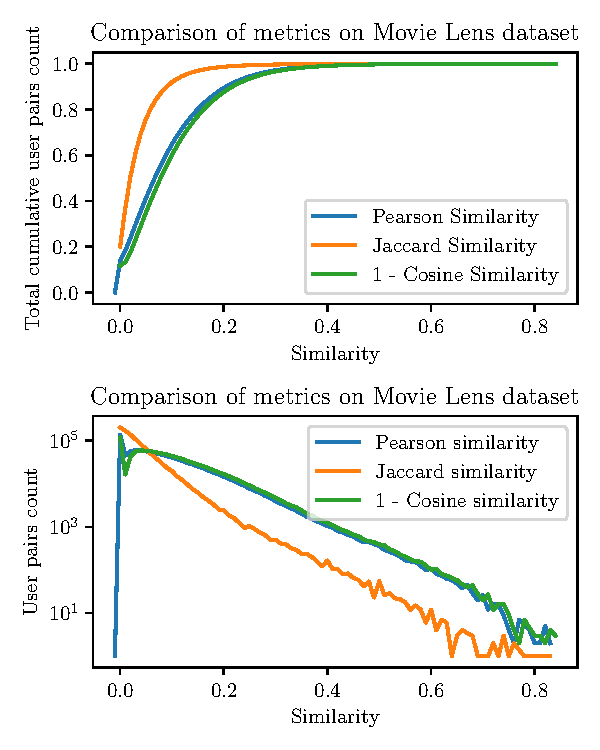
\includegraphics{img/figures/similarity_metrics.pdf}
    \caption{Comparison of similarity metrics on Movie Lens dataset.}
    \label{fig:similarity_metrics}
\end{figure}

We have compared the similarity metrics on a random sample of 1 million user pairs on \ref{fig:similarity_metrics}. Initially, we wanted to select Pearson Correlation Coefficient based on the before-mentioned stability, but interestingly, PCC and the Cosine similarity overlap substantially. This is due to the ratings being very sparse, which causes the means in PCC calculations to be close to 0, which corresponds to the Cosine similarity. Further, PCC and Cosine similarity, on average, have more samples with higher similarity and fewer samples with lower similarity. We, therefore, select Cosine similarity as our similarity metric due to its similarity to PCC and better properties than Jaccard similarity.

Now, we have a method of determining the similarity between two users. Further, we need to know how to modulate the amount of similarity in the group. There are many interesting ways how to create synthetic groups. Let us now present some of them.

Some of the possible types of group creation:
\begin{itemize}
    \item \textbf{Random:}
        Randomly sample without replacement from the user pool.
        
    \item \textbf{Similar:}
        Select one user randomly as a pivot, then fill in the remaining group spots with users that are as similar as possible. This basically is the k-nearest neighbors algorithm. The problem with this approach is that very rarely do we encounter situations like this in the real world. Another problem is that selecting the most similar users is computationally expensive as we need to compute the similarity between the pivot and every other user in the dataset, which is not ideal for the size of our data.
        
    \item \textbf{Somehow similar, with outliers:}
        One other way how to relax the similarity is to randomly select a pivot user and then select the nearest neighbors only from a random subset of the whole user pool. This way, we still get pretty similar users and do not need to perform so much computation.
        
        Another idea would be to select the next candidate based on the similarity to the last selected user instead of the pivot. In a way, we are creating a chain of users based on the similarity of the individual links(users). This way, we could create more variable preferences among the group members with still overlapping user-item interactions.
        
        Additionally, instead of selecting top-k similar users, we can make random steps in the similarity ordering, such as if we have 1000 most similar users ordered by the similarity metric, we do not need to take the top-k best ones, but for example, 100th most similar, 200th most similar and so on.
        
        Further, instead of a top-k, we can select users based on a weighted probability generated from the similarity or the ordering of all the candidate members.
        
    \item \textbf{Similar to the whole group:}
        Instead of selecting candidates similar to a single primary user, we can select the following group members to incrementally be similar to group members already assigned, either by aggregating the ratings or by, for example, Borda count. This has the advantage of easier candidate selection due to a bigger possible preference overlap. However, it has the disadvantage of needing to perform more similarity computations after each member selection.
        
    \item \textbf{Dissimilar:}
        Apart from finding group members based on being as similar as possible, we can also try to create as dissimilar groups as possible. Here we can randomly select a first user and then select a following user, which is as little similar as possible. Next, instead of selecting another user in the same way, we can calculate the dissimilarity of all other uses with the joined preference of the users already selected for the group and, again, select the most dissimilar one.
\end{itemize}


% -------------------------------------------------------------------------------------
\subsection{Selected approach}
% -------------------------------------------------------------------------------------
Let us now specify, in detail, the methods that we use and how we set the required parameters.

The simplest and most convenient option would be to calculate the similarity matrix for all users and then select groups based on this single calculation. However, this matrix can become pretty huge with the growing number of users. Let us assume our worst case of 1,000,000 users of the Spotify dataset. Then we will have $10^{12}/2$ similarity calculations that need to be processed and stored. This becomes difficult to manage as the amount of memory needed would be around the order of terabytes and the time needed for processing on the order of hours or days. We, therefore, opt for an iterative approach, where we randomly select only a smaller subset of potential group members and select the actual group members from this smaller group instead of the whole user pool. This can lead to calculating the users' similarity multiple times, but that situation is somewhat unlikely, and in total, we will save orders of magnitude worth of similarity calculation (potentially depending on the number of groups we want to generate).

\subsubsection{At random}
A straightforward approach that generates groups with very distinct user preferences. We select the desired amount of users for one group from the user pool and assign them together. Then repeat with the whole user pool (not removing the selected members) again.

\subsubsection{Similar groups with top-k selection}
We select one user as a pivot of the group at random. Next, we select some number of users randomly from the dataset as candidates and calculate the similarity between the pivot and each of the selected user candidates. Next, we select the top-N most similar users to the pivot where N is the desired group size - 1 and fill in the rest of the group with these top-N most similar.

This ensures that there will be pressure towards similarity using the top-K mechanism as well as some variety due to the random selection of candidates.

\subsubsection{Similar groups with probability respecting similarity (PRS)}
We perform the same random selection as in the previous method for similar groups but with a different procedure in the second step of selection from the candidates. We want to select a candidate with a probability that corresponds to their similarity with the pivot user and decreases quite heavily to ensure that there is still enough push toward selecting similar users.

\begin{figure}[ht!]
    \centering
    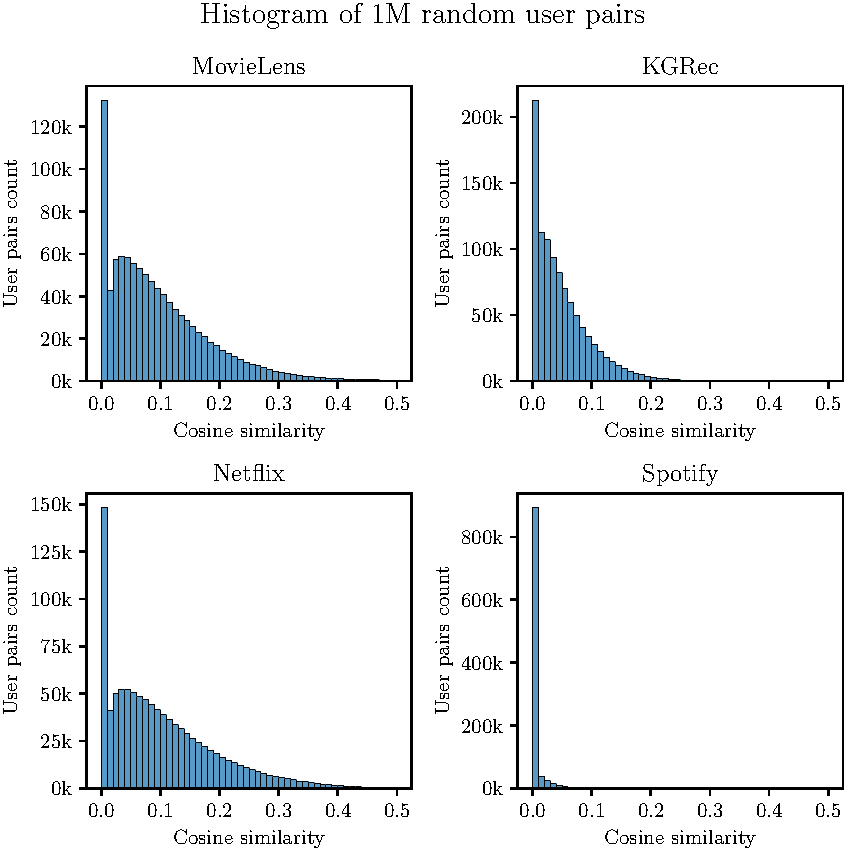
\includegraphics{img/figures/histogram_cosine_all.pdf}
    \caption{Histogram of cosine similarity of 1 million random user pairs from Movie Lens dataset.}
    \label{fig:cosine_all_histogram}
\end{figure}

Due to the exponentially decreasing number of users with higher similarity scores, as can be seen in Figure \ref{fig:similarity_metrics} and detail in Figure \ref{fig:cosine_all_histogram}, we need to ensure that potential group members with higher similarity still retain overall higher probability of being selected. We can do that by presetting the desired probability to each cosine similarity group and then dividing this probability by the average number of user pairs in that similarity group.

Unfortunately, we do not have the precise average number of user pairs, which would require us to compute the similarity between all possible pairs. We can get a good estimation by sampling some user pairs and calculating the ratio between the size of the group and the number of total samples. Sample of size 1 million on all datasets can be seen in Figure \ref{fig:cosine_all_histogram}.


In order to avoid deciding on the correct amount of bins to split the data into and how to smooth and sample from the bins, we have selected to model the expected cosine similarity probability density function minimizing the L2 norm. That allows us then to calculate what is the expected amount of samples in a small neighborhood. For Movie Lens, we have selected an exponential distribution with parameter $\lambda=0.08918$. This distribution models our underlying data quite well. Comparison can be found in Table \ref{table:5.3_modeled_comparison}. A most important portion of samples between 0.4 to 0.8, where most of the members with the highest chance of being selected will fall, seems to be modeled quite precisely.
Then we can express the average expected amount of similarity pairs with similarity of $x$ in some small constant-sized neighborhood of size $NS$ to be:
\begin{equation}
    expectedSRI\footnote{expected sample ratio on interval}(x, N, \lambda) = CDF(exp(\lambda), x + N) - CDF(exp(\lambda), x),
\end{equation}
where CDF stands for the cumulative distribution function of exponential distribution with the $\lambda$ parameter of $0.08918$. 

\begin{table}[!ht]
    \centering
    \begin{tabular}{ c | c | c}
       cosine sim. & sampled data & $exp(\lambda=0.08918)$ \\
        \hline
        $\left[ 0.0, 0.1\right)$ & 600,716 & 674,139 \\
        $\left[ 0.1, 0.2\right)$ & 275,099 & 219,675 \\
        $\left[ 0.2, 0.3\right)$ & 90,355 & 71,583 \\
        $\left[ 0.3, 0.4\right)$ & 24,265 & 23,326 \\
        $\left[ 0.4, 0.5\right)$ & 6,660 & 7,601 \\
        $\left[ 0.5, 0.6\right)$ & 2,181 & 2,476 \\
        $\left[ 0.6, 0.7\right)$ & 602 & 807 \\
        $\left[ 0.7, 0.8\right)$ & 110 & 263 \\
        $\left[ 0.8, 0.9\right)$ & 12 & 85 \\
        $\left[ 0.9, 1.0\right]$ & 0 & 27 \\d
        total & 1,000,000 & 999,982
            
    \end{tabular}
    % \caption[Rating of selected GRS datasets.]{Rating of selected GRS datasets. Note for 'n/a' - we were unable to download the dataset, therefore unable to asses this criteria}
    \caption{Comparison of histograms of data sampled from the dataset and the created data model.}
    \label{table:5.3_modeled_comparison}
\end{table}

However, we are not necessarily interested in the expected amount of samples on an interval. The main requirement is to have a ratio of expected occurrence between the sampled similarities. We are not interested in the actual value. Therefore approach using a probability density function of the modeled distribution is better. We can calculate the ratio as follows:

\begin{equation}
    expectedSampleRatio(x, \lambda) = pdf(exp(\lambda), x) = \lambda e ^{-\lambda x},
\end{equation}
where pdf represents the probability density function.

Next, we need to know how to scale the actual similarity. We would like to have a non-linear difference between samples. If sample $A$ has a similarity higher than sample $B$ by $0.1$, then we would like to have sample $A$ be selected twice as likely. Further, we can generalize the difference as parameter $D$ and the multiplying factor as $M$.

We get:
\begin{equation}
    scale(x, D, M) = M^{\frac{1}{D}x} = M^{\frac{x}{D}},
\end{equation}
where for doubling the probability, every 0.1 similarity difference will become:

\begin{equation}
    scale(x, 2, 0.1) = 2^{\frac{x}{0.1}} = 2^{10x}.
\end{equation}


\begin{equation}\label{eq:weight}
    \begin{aligned}
        weight(x, D, M, \lambda) &= \frac{scale(x, D, M)}{expectedSampleRatio(x, \lambda)} \\
        & = \frac{M^{\frac{x}{D}}}{\lambda e ^{-\lambda x}}
    \end{aligned}
\end{equation}

Parameter D in scale calculation has a significant impact on scaling. Unfortunately, it needs to be tuned to each dataset separately due to the different rating distributions, as shown in Figure \ref{fig:cosine_all_histogram}. Through experimentation, we have observed that the value of 0.1 seems to give us good results on every dataset apart for Spotify, where the width needs to be shortened substantially. We solve this situation by setting the parameter to the width of the interquartile range of the sampled ratings. In other words, we set it to the width of the middle 50\% mass for each dataset. We can see the resulting parameters for each dataset based on 1 million random user pairs in Table \ref{table:5.3_interquartile_width}. 

\begin{table}[!ht]
    \centering
    \begin{tabular}{ l l}
        dataset & \makecell[l]{interquartile \\ width (D)} \\
        \hline
        MovieLens & 0.104 \\
        KGRec & 0.057 \\
        Netflix & 0.114 \\
        Spotify & 0.025
            
    \end{tabular}
    \caption{Scaling width parameter based on the interquartile range of each dataset.}
    \label{table:5.3_interquartile_width}
\end{table}



\begin{algorithm}
	\caption{Generate groups with probability respecting similarity}
	\begin{algorithmic}[1]
	    \State Select scaling parameter $M$ and the desired amount of samples $S$ and amount of candidates $C$
	
	    \vspace{3mm}
	
	    \For {Desired number of samples $S$}
    	    \State Select random pair for users $u1$ and $u2$ from the user-pool
    	    \State Calculate similarity of $u1$ and $u2$ and store it
	    \EndFor
	    \State Fit an exponential distribution to the stored values
	    \State Calculate the width between 25th and 75th quartile as parameter D
	    \State Get its parameter $\lambda$
	    
	    \vspace{3mm}
	    
	    \For {Number of desired groups}
    	    \State Select 1 user $uCaptain$ from the user-pool as main user
    	    \State Select $C$ random users as $uCandidates$ from the user-pool
    	    \For {Each user $u$ from $uCandidates$}
    	        \State Calculate similarity between $uCaptain$ and $u$ as $sim$
    	        \State Calculate random candidate weight with (Eq. 5.8):
    	        \State $weight$ = scale($sim$, D, M) / expectedSampleRatio($sim$, $\lambda$)
    	    \EndFor
    	    \For{ Desired group size - 1}
    	    \State Perform weighted random selection on the candidates using the weights
    	    \State Add the selected user to the group and remove it from the candidates
    	    \EndFor
        \EndFor
	\end{algorithmic}
	\label{alg:create_sim_groups}
\end{algorithm} 



This gives us a framework for assigning each candidate member a weight by which we can perform a weighted random choice and therefore introduce more variability into the group selection process. The entire equation for a sample's weight can be calculated with Equation \ref{eq:weight}. Further, we describe the whole group generation process in Algorithm \ref{alg:create_sim_groups}.










% Pearson Correlation Coefficient due to its stable performance as mentioned in \cite{similarity_measures_comparason},  and due to its wide use among the recommender system domain.

% \textbf{Pearson correlation coefficient} for two vectors $X$ and $Y$ can be computed as follows:
% \begin{equation}
%     P(X,Y) = \frac{\text{cov}(X,Y)}{\sigma_x \sigma_y}
%     = \frac{{}\sum_{i=1}^{n} (x_i - \overline{x})(y_i - \overline{y})}{\sqrt{\sum_{i=1}^{n} (x_i - \overline{x})^2(y_i - \overline{y})^2}},
% \end{equation}
% where $cov$ is the covariance, and $\sigma$ is the standard deviation.

% Further we have selected \textbf{Jaccard similarity} due to its simplicity:
% \begin{equation}
%     J(X,Y) = \frac{|X \cap Y|}{|X \cup Y|} = \frac{|X \cap Y|}{|X| + |Y| - |X \cap Y|}.
% \end{equation}
% It has a 

% -------------------------------------------------------------------------------------
\subsection{Evaluation of the generated groups} \label{subsec:04_creation_of_artificial_groups.evaluation}
% -------------------------------------------------------------------------------------

We have implemented and used the selected techniques to generate synthetic groups. Let us now evaluate the performance of each method. Next, we discuss the parameters of the generation process.

The random method is the simplest from the point of selecting parameters of the group creation. It does not have any.

Next, the top-k method, it only has a single parameter of the number of candidates from which we choose the actual group members. We have set the default number of candidates to 1000 due to the computational complexity rising linearly with the number of candidates.

Lastly, our PRS method. It has three parameters in total, where $\lambda$ is the parameter of the exponential distribution fitted to a sample of user similarities. D is the distance, and M is the multiplier factor of the scale ratio. We have set the distance to be 0.1, and we vary the multiplier factor from 0,5 to 4.

We aim to compare the mean inter-group similarity. First, we define a subset of size $n$ of set $S$ as

\begin{equation}
    R(S, n) := { x \in \mathcal{P}(S) : |x| = n},
    \end{equation}
where $\mathcal{P}$ is a powerset, a set of all subsets. 

Then we define the inter-group similarity, which represents the mean of similarity between all tuples in the group as
\begin{equation}
    intergroupSimilarity(G) = \frac{1}{|R(G,2)|}\mathlarger{\sum}_{\{a,b\} \in R(G,2)}  cos(a,b).
\end{equation}


\begin{figure}[ht!]
    \centering
    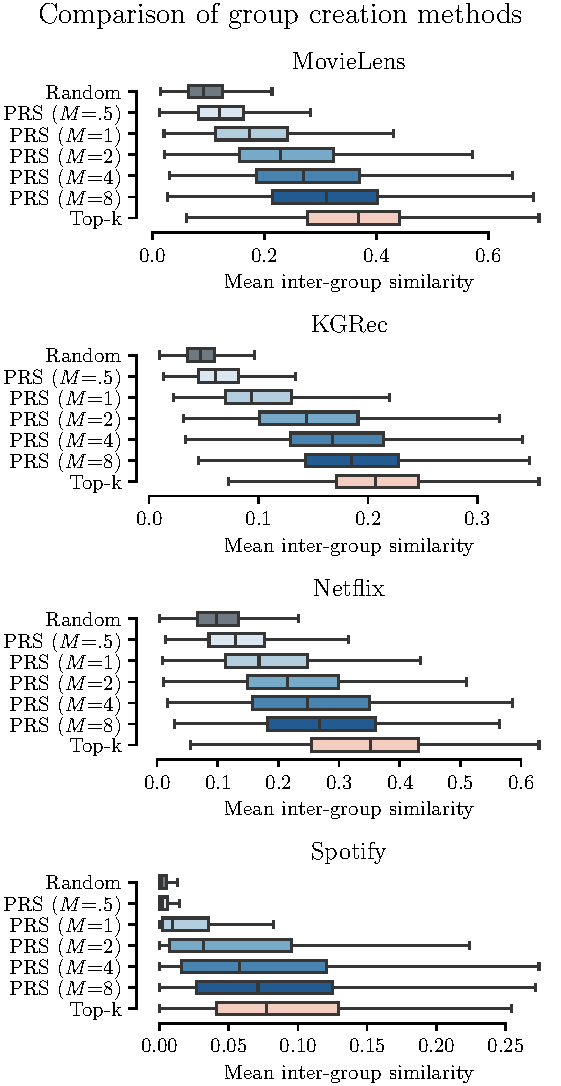
\includegraphics{img/figures/inter_group_means.pdf}
    \caption[Comparison of Random, Top-k and multiple variants of PRS group generation for group size of 5.]{Comparison of Random, Top-k and multiple variants of PRS group generation for group size of 5. The number of candidates for PRS and Top-k was 1000.}
    \label{fig:inter_group_means}
\end{figure}

With each group generation method, we have created 1000 groups of size 5. The resulting mean inter-group similarities can be seen in Figure \ref{fig:inter_group_means}. As expected, the random and top-k have the least and most mean inter-group similarity. With PRS, we have achieved the desired scaling of the mean inter-group similarity between the random and top-k. Furthermore, we see that PRS generates groups that are comparably or more varied in the similarity as top-. Other methods, which manage to create groups that utilize some similarity scaling, such as in \cite{GFAR-kaya2020} that select candidates based on their similarity with the pivot will not produce groups that vary in the inter-group similarity.

At first, PRS did not scale well on the Spotify dataset, with parameter D set to 0.1. The dataset has its similarity concentrated closer to zero. This is because most users (playlists) did not rate more than 30 items. The majority of ratings are between $0$ and $0.1$; therefore, we need to set the scaling width to a lower value to compensate for this. Based on this, we have introduced the technique of setting the D parameter to the width of the interquartile range, which solves the issue and decreases the number of parameters that need to be tuned to only one - the scaling parameter M. 

In conclusion, we are satisfied with the PRS technique. It provides us with a method of reliable generation of groups of varying inter-group similarity, which are more heterogenous and therefore closer to reality than selecting group members solely based on the desired similarity.

% \section{Dataset tool} \label{sec:dataset_tool}

% We have created a Python CLI tool that allows users to download and process datasets mentioned in \ref{sec:single_user_datasets} and create artificial groups with methods described in \ref{sec:creation_of_artificial_groups}.

% \todo[inline]{add parameters, screenshot and requrements}

% - clanky co cituji gfar vytvarely umele skupiny, prozkoumat,
% - lada clanek jednotlive popisy
% - porovnani prozkoumani a nasledne shrnuti/vylepseni
